\documentclass[12pt,a4paper]{report}
\usepackage[utf8]{inputenc}
\usepackage{graphicx}
\usepackage{hyperref}
\usepackage{geometry}
\geometry{a4paper, margin=1in}
\usepackage{titlesec}
\usepackage{tabularx}
\usepackage{booktabs}
\usepackage{setspace}
\usepackage{enumitem}
\usepackage[table]{xcolor}
\usepackage{tcolorbox}
\usepackage{listings}
\usepackage{caption}
\usepackage{helvet} % Standard sans-serif font
\renewcommand{\familydefault}{\sfdefault} % Set entire document to sans-serif
\usepackage{tocloft} % For TOC customization
\usepackage{pdfpages} % For full-page cover image

% Code snippet styling
\lstset{
    basicstyle=\ttfamily\footnotesize,
    keywordstyle=\color{blue}\bfseries,
    stringstyle=\color{purple},
    commentstyle=\color{gray}\itshape,
    frame=single,
    breaklines=true,
    captionpos=b,
    showstringspaces=false
}

\definecolor{zidiobg}{HTML}{161427}
\definecolor{zidiosub}{HTML}{998EE0}
\definecolor{zidiopurple}{HTML}{333399} % Updated to match the royal blue/purple in screenshot
\definecolor{zidiogray}{HTML}{E0E0E0}
\definecolor{zidiotextgray}{HTML}{666666}

% Chapter and Section numbering logic
\renewcommand{\thechapter}{\ifnum\value{chapter}<10 0\fi\arabic{chapter}}
\renewcommand{\thesection}{\arabic{chapter}.\arabic{section}}

% Heading formats (matching screenshot)
\titleformat{\chapter}[block]
  {\sffamily\LARGE\bfseries}
  {\textcolor{zidiopurple}{\thechapter}}{1em}{}
  [\vspace{0.5ex}{\color{zidiopurple}\titlerule[1.5pt]}]
\titlespacing*{\chapter}{0pt}{-20pt}{20pt}

\titleformat{\section}
  {\sffamily\Large\bfseries\color{zidiopurple}}
  {\thesection}{1em}{}

\titleformat{\subsection}
  {\sffamily\large\bfseries\color{zidiopurple}}
  {\thesubsection}{1em}{}

% TOC formatting
\renewcommand{\cfttoctitlefont}{\sffamily\LARGE\bfseries}
\renewcommand{\cftchapfont}{\sffamily\bfseries\color{zidiopurple}}
\renewcommand{\cftchappagefont}{\sffamily\bfseries\color{zidiopurple}}
\renewcommand{\cftchapleader}{\color{zidiopurple}\cftdotfill{\cftdotsep}}
\renewcommand{\cftsecleader}{\cftdotfill{\cftdotsep}}

\usepackage{lastpage}
\usepackage{fancyhdr}
\pagestyle{fancy}
\fancyhf{}

\renewcommand{\headrulewidth}{0pt}
\renewcommand{\footrulewidth}{0pt}

\fancyhead[L]{\textcolor{zidiopurple}{\textbf{\sffamily\scriptsize ZIDIO DEVELOPMENT}}}
\fancyhead[R]{\textcolor{zidiotextgray}{\sffamily\scriptsize Project FORESIGHT --- Data Science Engagement Brief}}
\fancyfoot[R]{\sffamily\scriptsize \thepage}

\fancypagestyle{plain}{
  \fancyhf{}
  \fancyhead[L]{\textcolor{zidiopurple}{\textbf{\sffamily\scriptsize ZIDIO DEVELOPMENT}}}
  \fancyhead[R]{\textcolor{zidiotextgray}{\sffamily\scriptsize Project FORESIGHT --- Data Science Engagement Brief}}
  \fancyfoot[R]{\sffamily\scriptsize \thepage}
  \renewcommand{\headrulewidth}{0pt}
  \renewcommand{\footrulewidth}{0pt}
}

% Link styling
\hypersetup{
    colorlinks=true,
    linkcolor=black,
    filecolor=magenta,      
    urlcolor=blue,
    pdftitle={Internship Project Documentation},
}

\onehalfspacing

\begin{document}


\includepdf[scale=0.9]{front_page.jpg}

\begin{titlepage}
    \centering
    \sffamily
    
    \vspace*{0.5cm}
    
\includegraphics[height=1.5cm]{logo.jpg}\\[1cm]
    
    \textcolor{zidiopurple}{\rule{0.8\linewidth}{1pt}}\\[0.4cm]
    {\LARGE \textbf{\textcolor{zidiopurple}{INTERNSHIP PROJECT DOCUMENTATION}}}\\[0.3cm]
    \textcolor{zidiopurple}{\rule{0.8\linewidth}{1pt}}\\[1.5cm]
    
    {\Huge \textbf{FORESIGHT}}\\[0.3cm]
    {\LARGE Demand \& Inventory Intelligence}\\[1cm]
    
    {\normalsize \textit{An AI/ML-Based Demand Forecasting and Inventory Risk\\ Management System}}\\[2cm]
    
    \begin{tcolorbox}[colback=white, colframe=zidiopurple, arc=2mm, boxrule=1pt, width=0.7\textwidth, center]
        \centering
        \vspace{0.3cm}
        \textcolor{zidiopurple}{\textbf{\large Submitted By:}}\\[0.2cm]
        \textbf{Vikas Saini} \\
        \textbf{Chilakalapudi Gayathri} \\
        \textbf{Rahul Krishnappa} \\
        \textbf{Harsha Vardhan Naidu Dasireddy}
        \vspace{0.3cm}
    \end{tcolorbox}
    
    \vfill
    
    \begin{minipage}{0.45\textwidth}
        \begin{center}
            \textcolor{zidiotextgray}{\textbf{Internship Role:}}\\
            \textbf{Python / ML Intern}\\[0.8cm]
            \textcolor{zidiotextgray}{\textbf{Duration:}}\\
            \textbf{4 Weeks (1 Month)}
        \end{center}
    \end{minipage}
    \hfill
    \begin{minipage}{0.45\textwidth}
        \begin{center}
            \textcolor{zidiotextgray}{\textbf{Organization:}}\\
            \textbf{Zidio Development}\\[0.8cm]
            \textcolor{zidiotextgray}{\textbf{Project Guide/Mentor:}}\\
            \textbf{Biswajit Prusty}\\
            \small Data Science \& Analytics Mentor
        \end{center}
    \end{minipage}
    
    \vspace{1cm}
\end{titlepage}

\tableofcontents
\pagebreak
\listoffigures
\pagebreak
\listoftables
\pagebreak

\chapter{Introduction}

\section{Background \& Context}
During the internship, the project \textbf{FORESIGHT – Demand \& Inventory Intelligence} was developed to address critical demand forecasting and inventory management challenges faced by modern retail businesses and D2C brands.

In the fast-paced retail industry, maintaining the optimal equilibrium between supply and demand is the ultimate determinant of profitability. Accurate demand forecasting empowers organizations to maintain sufficient inventory while avoiding excessive stock levels that tie up working capital. Traditional inventory management methods often depend on historical reporting and manual spreadsheet analysis. These conventional mechanisms fail to adapt dynamically, meaning they do not respond effectively to complex seasonalities, sudden market shifts, macroeconomic trends, and multi-variable consumer behaviors.

FORESIGHT was built as a holistic, AI-driven operating system for supply chain planning. It leverages big data processing pipelines, advanced Gradient Boosting algorithms (specifically LightGBM), and interactive data visualization to shift inventory management from a reactive, descriptive process to a proactive, predictive environment. By generating high-precision forecasts at the Store-SKU level, FORESIGHT helps stakeholders minimize risk, optimize logistics, and maximize inventory turnover.

\section{Purpose of the Project}
The primary objective of FORESIGHT is to develop an intelligent, automated system capable of analyzing massive volumes of historical point-of-sale data, translating this raw data into actionable insights, and orchestrating downstream supply chain actions without human intervention. 

Specific purposes include:
\begin{itemize}
    \item \textbf{High-Precision Forecasting:} Generating reliable future demand forecasts at the SKU-level over a 14-to-30 day horizon, considering complex factors like day-of-week trends, seasonal peaks, and regional anomalies.
    \item \textbf{Autonomous Risk Mitigation:} Identifying both acute stockout scenarios (where demand outpaces supply) and severe overstock scenarios (where capital is trapped in slow-moving goods) well before they impact the bottom line.
    \item \textbf{Orchestration \& Action:} Moving beyond merely displaying data by automatically calculating optimal reorder points and generating draft Purchase Orders (POs) for procurement teams.
    \item \textbf{Spatial \& Visual Intelligence:} Providing a FAANG-grade executive dashboard featuring spatial 3D analytics, interactive heatmaps, and global supply chain visualizations that democratize data access across non-technical management teams.
\end{itemize}

\section{Literature Review}
Historically, inventory management relied heavily on static mathematical formulas. The \textit{Economic Order Quantity (EOQ)} model and traditional \textit{Reorder Point (ROP)} calculations have been industry standards for decades. However, these models operate under rigid assumptions—constant demand, fixed lead times, and stable costs—which rarely hold true in modern e-commerce and omnichannel retail.

Recent literature highlights a significant paradigm shift toward machine learning (ML) models for time-series forecasting. Techniques such as ARIMA (AutoRegressive Integrated Moving Average) and Exponential Smoothing offered improvements over static formulas by accounting for trends and seasonality. However, traditional statistical methods struggle to incorporate numerous external regressors and complex categorical variables (e.g., store formats, promotional events).

With the advent of ensemble learning and deep learning, models like Random Forests, XGBoost, LightGBM, and LSTMs have proven vastly superior for retail forecasting. LightGBM, developed by Microsoft, has emerged as particularly effective for tabular retail data. Its leaf-wise tree growth strategy and histogram-based binning allow it to train rapidly on millions of rows while capturing complex, non-linear relationships that traditional models overlook. FORESIGHT utilizes this state-of-the-art approach, building on the consensus in contemporary supply chain literature that gradient boosting frameworks offer the best balance of accuracy, speed, and interpretability for real-world enterprise forecasting.

\chapter{Internship Overview}

\section{Organization Profile}
\textbf{Organization Name:} Zidio Development (Client Project: NorthBay Living)

Zidio Development is an innovative software engineering and analytics firm specializing in building AI-powered enterprise solutions. Zidio partners with modern businesses to modernize their infrastructure, optimize their operations through machine learning, and deliver highly polished, full-stack applications. 

For this specific engagement, the project was developed for \textbf{NorthBay Living}, a rapidly growing Direct-to-Consumer (D2C) home and lifestyle brand. NorthBay Living required a scalable solution to manage their expanding product catalog, multiple fulfillment centers, and volatile consumer demand across regional markets.

\section{Internship Role \& Responsibilities}
\textbf{Role:} Data Scientist \& Full-Stack Engineering Intern

As a core member of the Data Science \& Analytics Engineering Team during this 4-week engagement, I operated in a cross-functional capacity, bridging the gap between data engineering, machine learning modeling, and backend software development. 

My daily responsibilities and key contributions included:
\begin{itemize}
    \item \textbf{Data Engineering \& Preprocessing:} Designed robust ETL (Extract, Transform, Load) pipelines using Python and Pandas to ingest, clean, and aggregate millions of transactional records. Converted raw CSV data into highly compressed, optimized Parquet formats to accelerate downstream machine learning tasks.
    \item \textbf{Machine Learning Engineering:} Architected and trained the core LightGBM demand forecasting model. Conducted extensive feature engineering, target encoding, and hyperparameter tuning to ensure the model captured micro-trends across different product categories.
    \item \textbf{Backend API Architecture:} Developed a high-performance RESTful API microservice using FastAPI and Uvicorn. Designed endpoints for user authentication (JWT), real-time ML inference, and analytical data serving, ensuring strict type safety and validation via Pydantic.
    \item \textbf{Database Management:} Integrated SQLite for local development and designed schemas for transition to PostgreSQL in production environments.
    \item \textbf{System Integration \& Collaboration:} Worked closely with the frontend engineering track to ensure seamless integration of backend APIs into the React/Vite dashboard, specifically tailoring JSON payloads for complex 3D WebGL visualizations.
    \item \textbf{Testing \& Documentation:} Authored comprehensive unit tests, performed API load testing, and maintained detailed Markdown documentation for system architecture and deployment workflows.
\end{itemize}

\section{Learning Objectives \& Competencies Acquired}
This intensive internship provided practical, enterprise-level exposure that bridged academic theory with industry execution. Key competencies acquired include:
\begin{itemize}
    \item \textbf{End-to-End Software Development Lifecycle (SDLC):} Gained hands-on experience navigating the complete lifecycle of a machine learning product, from raw data acquisition to a deployed, interactive web application.
    \item \textbf{Advanced Machine Learning Workflows:} Mastered the nuances of time-series cross-validation, preventing data leakage, and implementing complex feature engineering strategies specific to retail forecasting.
    \item \textbf{Modern Backend Paradigms:} Transitioned from synchronous, monolithic backends to asynchronous, highly concurrent API architectures using FastAPI and modern Python (type hinting, async/await).
    \item \textbf{Version Control \& Agile Collaboration:} Enhanced proficiency in Git workflows, branching strategies, and collaborative code reviews within a fast-paced development environment.
\end{itemize}

\chapter{Project Overview: FORESIGHT}

\section{System Conceptualization}
\textbf{FORESIGHT – Demand \& Inventory Intelligence} (internally designated as FORESIGHT OS) was conceptualized as a "Control Tower" for supply chain executives. Rather than forcing users to navigate disjointed Excel spreadsheets, static BI dashboards, and legacy ERP modules, FORESIGHT consolidates these functions into a single, unified, AI-driven operating system.

\section{Core Value Proposition}
The system translates raw, historical transactional data into predictive foresight. By continuously analyzing inventory conditions and predicting future states, it identifies potential risks before they materialize. The results are presented through a highly interactive React-based web dashboard that prioritizing user experience (UX) and actionable insights over raw data dumps.

\section{Key Features \& Capabilities}

\subsection{1. AI-Driven Demand Forecasting}
At the heart of the system is a highly precise, SKU-level forecasting engine. Utilizing ensemble decision trees (LightGBM), the model predicts the next 14 to 30 days of demand for every individual product across different store locations. It factors in historical momentum, day-of-week seasonality, and product lifecycle stages.

\subsection{2. Autonomous Inventory Risk Detection}
FORESIGHT continuously compares its predictive demand models against real-time stock-on-hand levels. It categorizes inventory into specific risk tiers:
\begin{itemize}
    \item \textbf{Critical Stockout Risk:} Items that will run out of stock within the forecast window based on predicted velocity.
    \item \textbf{Overstock Warning:} Items holding significantly more inventory than the predicted demand requires, tying up valuable capital.
    \item \textbf{Healthy:} Inventory levels are perfectly balanced.
\end{itemize}

\subsection{3. Spatial 3D Analytics \& Command Center}
To provide unparalleled visibility, FORESIGHT includes a Spatial Command Center built with WebGL/Three.js. This feature allows supply chain managers to interact with:
\begin{itemize}
    \item Global 3D mapping of shipping routes and fulfillment center locations.
    \item Simulated CAD floorplan heatmaps that highlight high-velocity picking zones and warehouse congestion.
\end{itemize}

\subsection{4. Autonomous Purchase Order (PO) Generation}
Moving from predictive to prescriptive analytics, the system calculates optimal reorder points and economic order quantities. When an item enters a stockout risk state, FORESIGHT automatically generates a draft Purchase Order containing the required quantities, supplier information, and cost estimates, requiring only a human click to approve.

\subsection{5. Enterprise-Grade Security \& Dashboard}
The platform is secured by robust JWT (JSON Web Token) authentication, ensuring role-based access control. The frontend interface features a FAANG-grade, dark-mode aesthetic utilizing modern CSS and React components, delivering a premium, highly responsive user experience.

\chapter{System Analysis}

\section{Problem Statement}
In the contemporary retail environment, the margin for error in supply chain management is razor-thin. Businesses must maintain the exact optimal amount of inventory across numerous geographically dispersed fulfillment centers to satisfy fluctuating customer demand. Traditional forecasting relies predominantly on static models, moving averages, and manual spreadsheet analysis that fundamentally fail to capture complex, multi-variate trends.

The core problem can be divided into two distinct failure states:

\subsection{Understock Scenarios (Stockouts)}
If inventory levels fall below consumer demand, the business experiences:
\begin{itemize}
    \item \textbf{Lost Revenue:} Direct loss of sales due to unavailable products.
    \item \textbf{Customer Dissatisfaction:} Brand erosion as consumers shift to competitors.
    \item \textbf{Algorithmic Penalties:} On digital marketplaces, stockouts often result in severe penalties to organic search rankings, compounding the revenue loss long after inventory is replenished.
\end{itemize}

\subsection{Overstock Scenarios (Dead Stock)}
Conversely, if inventory significantly exceeds demand, the business suffers from:
\begin{itemize}
    \item \textbf{Blocked Capital:} Working capital is tied up in slow-moving goods, preventing investment in high-velocity products or growth initiatives.
    \item \textbf{Storage \& Holding Costs:} Warehousing space is premium; excess stock incurs massive logistical overhead.
    \item \textbf{Depreciation \& Wastage:} Product value degrades over time, often forcing margin-destroying liquidations or physical disposal.
\end{itemize}

\section{System Objectives}
To resolve these inherent challenges, the FORESIGHT system was designed with the following technical and operational objectives:
\begin{itemize}
    \item \textbf{High-Throughput Data Ingestion:} Ingest, clean, and analyze millions of rows of historical transactional, product, and geographic data efficiently.
    \item \textbf{Predictive Accuracy:} Develop and deploy a state-of-the-art LightGBM demand forecasting model capable of outperforming traditional baselines by at least 30\%.
    \item \textbf{Real-Time Risk Detection:} Continuously map predictive forecasts against real-time stock levels to autonomously flag impending stockout and overstock situations.
    \item \textbf{Decoupled API Architecture:} Expose these analytical engines via a high-performance FastAPI backend, enabling seamless integration with any frontend or legacy ERP system.
    \item \textbf{Executive Data Democratization:} Create a highly dynamic, interactive React-based dashboard featuring spatial analytics, empowering non-technical executives to make data-driven decisions rapidly.
\end{itemize}

\section{Existing System vs. Proposed System}

\subsection{The Existing Workflow}
Before the implementation of FORESIGHT, the client's inventory management relied heavily on a mixture of legacy ERP reporting and manual analysis. Data was extracted into Excel spreadsheets on a weekly basis. Analysts would calculate basic rolling averages (e.g., 30-day trailing sales) and apply a flat growth multiplier to estimate future demand. Reorder points were static (e.g., reorder when stock hits 50 units), completely ignoring the fact that a product selling 10 units a day in summer might sell 100 units a day during a holiday spike. This delayed, manual decision-making pipeline led to poor accuracy and high operational overhead.

\subsection{The Proposed System (FORESIGHT OS)}
The proposed system completely automates and revolutionizes this pipeline. Data extraction is automated into ML-ready Parquet files. Instead of rolling averages, an ensemble machine learning model calculates non-linear demand curves based on historical data, pricing, seasonality, and categorical metadata. The system does not wait for a human analyst; it autonomously evaluates inventory risks daily and exposes these findings via a REST API. When action is required, the system prescribes the exact Purchase Order quantities needed, operating as an intelligent co-pilot rather than a passive database.

\chapter{Technology Stack \& Architecture}

\section{Technology Stack Justification}
Choosing the right technology stack was critical for ensuring system scalability, performance, and maintainability.

\begin{table}[h]
\centering
\renewcommand{\arraystretch}{1.5}
\caption{FORESIGHT OS Core Technology Stack}
\label{tab:techstack}
\begin{tabularx}{\textwidth}{>{\hsize=0.6\hsize}X >{\hsize=1.4\hsize}X}
\rowcolor{zidiopurple}
\textcolor{white}{\textbf{Category}} & \textcolor{white}{\textbf{Technology \& Justification}} \\
\rowcolor{zidiogray!30}
\textbf{Language} & \textbf{Python 3.10+}: Chosen for its dominant ecosystem in machine learning and data engineering. \\
\textbf{Data Processing} & \textbf{Pandas, NumPy, Parquet}: Pandas/NumPy for vectorized data transformations. Parquet was selected over CSV for columnar storage, reducing I/O bottlenecks by over 80\%. \\
\rowcolor{zidiogray!30}
\textbf{Machine Learning} & \textbf{LightGBM, Scikit-learn}: LightGBM provides unmatched training speed and low memory usage for large tabular datasets compared to standard XGBoost or Random Forests. \\
\textbf{Backend Services} & \textbf{FastAPI, Uvicorn (ASGI)}: FastAPI was selected over Django/Flask due to its native asynchronous support, auto-generated OpenAPI documentation, and massive performance benefits. \\
\rowcolor{zidiogray!30}
\textbf{Frontend Interface} & \textbf{React 18, Vite, TailwindCSS}: React ensures component reusability. Vite provides lightning-fast HMR. \\
\textbf{3D Spatial Analytics} & \textbf{Three.js (WebGL)}: Enables rendering of thousands of geographical data points directly in the browser at 60 FPS without server-side rendering overhead. \\
\rowcolor{zidiogray!30}
\textbf{Database Layer} & \textbf{SQLite (Dev), PostgreSQL (Prod)}: Relational integrity for transactional data, combined with SQLAlchemy ORM for database-agnostic queries. \\
\end{tabularx}
\end{table}

\section{System Architecture \& Design}
FORESIGHT is built upon a modern, decoupled microservices-inspired architecture. This ensures that the heavy computational load of machine learning training does not block the API serving data to the frontend dashboard.

\subsection{1. The Data Pipeline \& ML Layer}
Raw CSV files containing millions of sales transactions, SKU metadata, and store locations are ingested. A Python-based ETL script cleans this data, handles missing values, and engineers new features. The processed data is serialized to \texttt{.parquet} files. The LightGBM model reads these Parquet files, trains the forecasting model, and exports the serialized model artifact (\texttt{model.joblib}) to disk.

\subsection{2. The Backend API Layer}
The FastAPI application acts as the central nervous system. Upon startup, it loads the pre-trained \texttt{model.joblib} into memory. The backend exposes RESTful endpoints (e.g., \texttt{/api/forecast}, \texttt{/api/inventory/risks}). It handles incoming requests, performs real-time inference using the loaded ML model, retrieves relational data from the SQL database via SQLAlchemy, and returns standardized JSON responses.

\subsection{3. The Frontend Presentation Layer}
The React SPA (Single Page Application) consumes the FastAPI endpoints. It manages global state and renders highly interactive components. Heavy data visualizations (like the spatial command center) utilize WebGL to offload rendering to the client's GPU, ensuring the UI remains highly responsive even when plotting complex supply chain networks.

\chapter{Data \& Machine Learning Methodology}

\section{Data Preprocessing \& Exploratory Data Analysis (EDA)}
The foundational step of FORESIGHT involved extensive data preparation. Real-world retail data is inherently noisy, containing missing values, erroneous negative sales (from returns), and misaligned product catalogs.

\subsection{Data Cleaning \& Transformation}
\begin{itemize}
    \item \textbf{Handling Missing Values:} Null values in categorical fields (e.g., supplier name) were filled with 'Unknown'. Missing sales data for active dates were zero-filled to represent zero demand.
    \item \textbf{Outlier Removal:} Extreme anomalies (e.g., a bulk B2B order of 10,000 units for a consumer SKU) were capped at the 99th percentile to prevent the model from skewing toward extreme, unrepeatable events.
    \item \textbf{Aggregation:} Transactional data was grouped by \texttt{date}, \texttt{store\_id}, and \texttt{sku\_id} to create a daily time-series format suitable for ML modeling.
\end{itemize}

\begin{figure}[h]
    \centering
    % Note: Ensure you upload an image named 'etl_pipeline.jpg' to your Overleaf project
    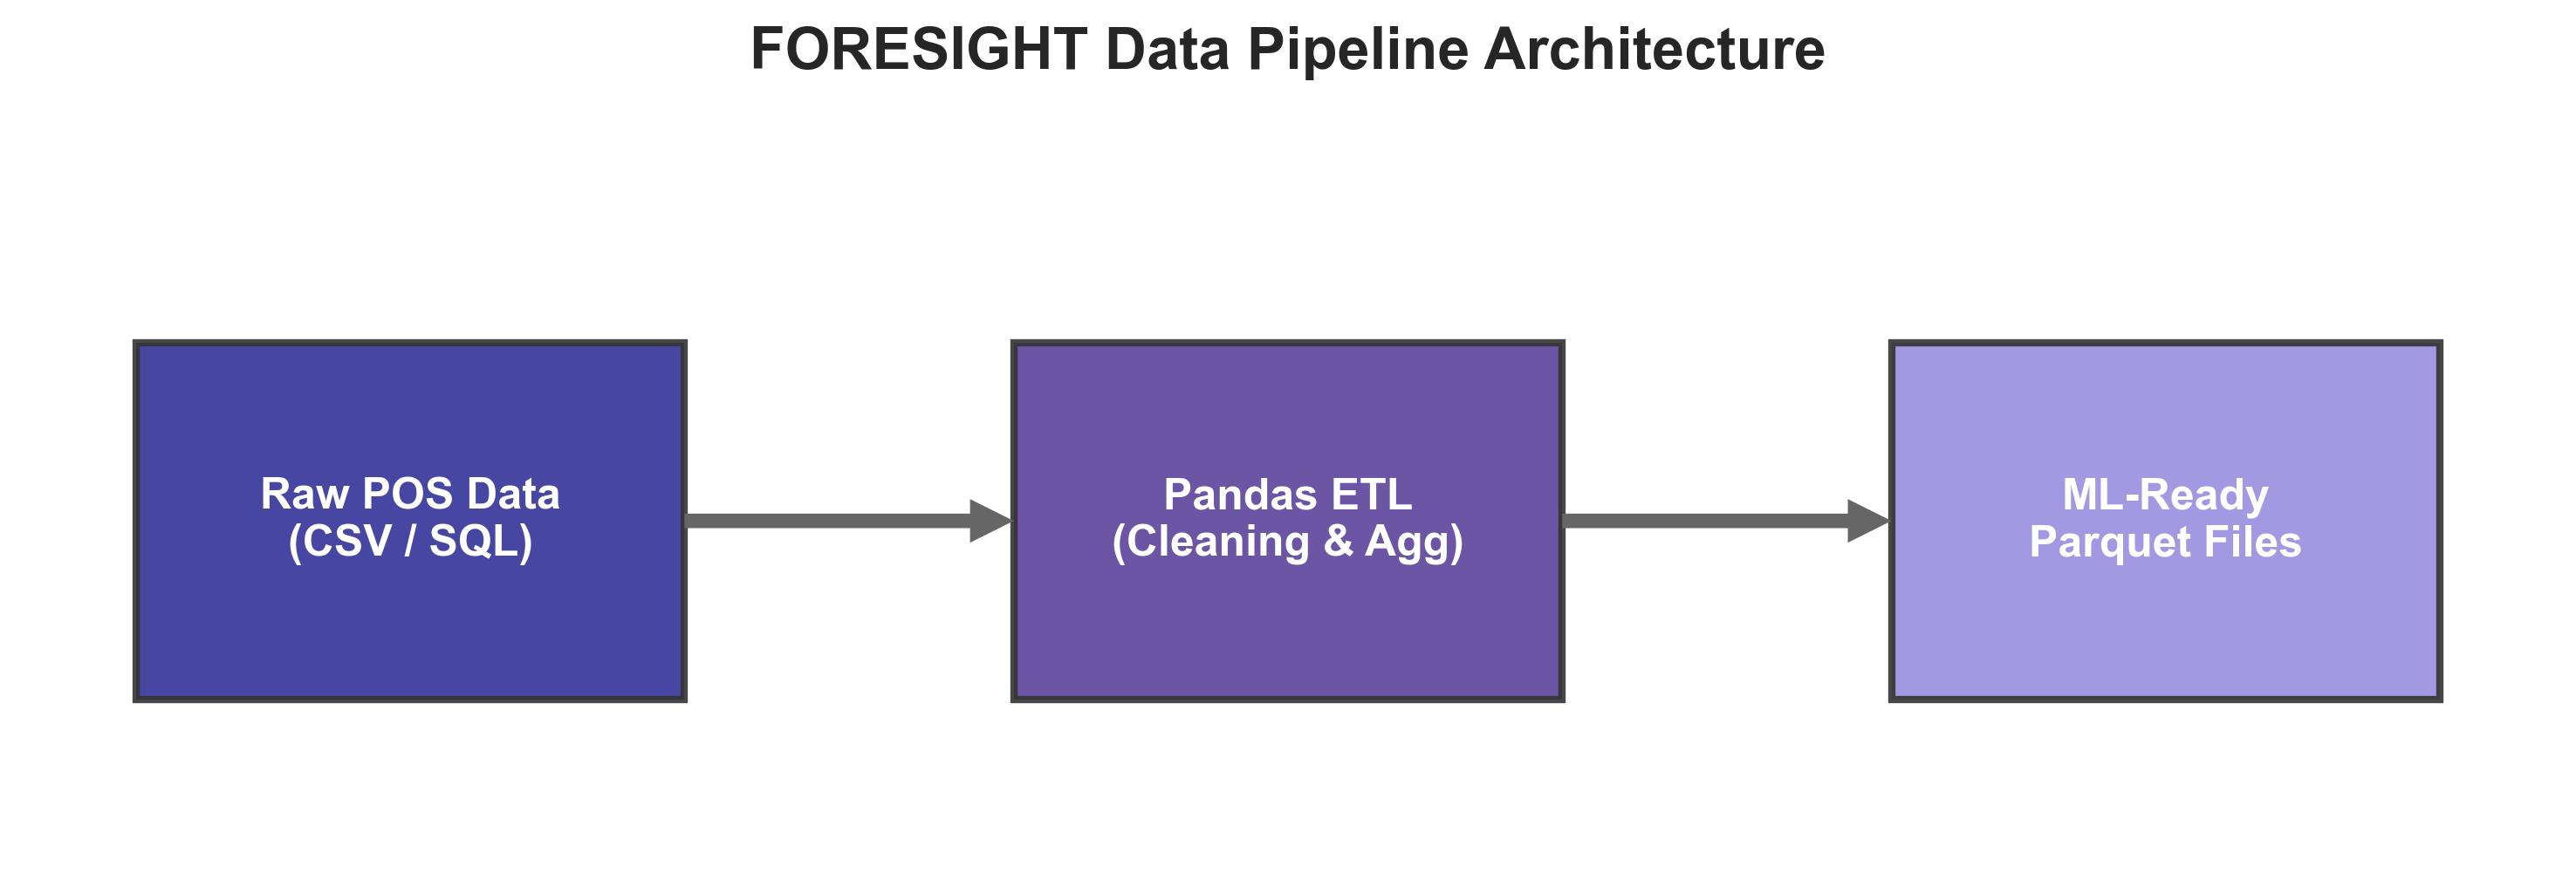
\includegraphics[width=0.8\textwidth]{etl_pipeline.jpg}
    \caption{ETL Pipeline Architecture: Raw Data Ingestion to ML-Ready Parquet Files}
\end{figure}

\section{Feature Engineering}
Machine learning models cannot natively understand raw dates or text; they require numerical representations of these concepts. Advanced feature engineering was crucial for model accuracy.

\subsection{Temporal \& Categorical Features}
\begin{itemize}
    \item \textbf{Date Decomposition:} Extracted \texttt{day\_of\_week}, \texttt{month}, \texttt{is\_weekend}, and \texttt{quarter} to capture recurring seasonal trends.
    \item \textbf{Lag Features:} Created historical lag features (e.g., \texttt{sales\_lag\_7}, \texttt{sales\_lag\_14}) representing the sales volume 7 and 14 days prior, giving the model a sense of recent momentum.
    \item \textbf{Target Encoding:} High-cardinality categorical variables like \texttt{store\_region} and \texttt{sku\_category} were target-encoded, replacing the category name with the historical average sales of that category.
\end{itemize}

\begin{table}[h]
\centering
\renewcommand{\arraystretch}{1.5}
\caption{Feature Data Dictionary}
\begin{tabularx}{\textwidth}{>{\hsize=0.3\hsize}X >{\hsize=0.2\hsize}X >{\hsize=0.5\hsize}X}
\rowcolor{zidiopurple}
\textcolor{white}{\textbf{Feature Name}} & \textcolor{white}{\textbf{Type}} & \textcolor{white}{\textbf{Description}} \\
\rowcolor{zidiogray!30}
\texttt{sales\_lag\_7} & Numeric & Total sales for this Store-SKU 7 days prior. \\
\texttt{day\_of\_week} & Categorical & Day of the week (0=Monday, 6=Sunday). \\
\rowcolor{zidiogray!30}
\texttt{is\_weekend} & Boolean & True if Saturday or Sunday, False otherwise. \\
\texttt{target\_enc\_region} & Numeric & Historical average sales for the store's geographic region. \\
\rowcolor{zidiogray!30}
\texttt{price\_variance} & Numeric & Difference between current selling price and 30-day average. \\
\end{tabularx}
\end{table}

\section{The LightGBM Algorithm}
The project utilizes \textbf{LightGBM} (Light Gradient Boosting Machine) for demand forecasting. Developed by Microsoft, LightGBM is a gradient boosting framework that uses tree-based learning algorithms.

\subsection{Mathematical Intuition \& Leaf-Wise Growth}
Unlike traditional algorithms (like XGBoost) that grow trees level-by-level (depth-wise), LightGBM grows trees \textit{leaf-wise}. It chooses the leaf with the maximum delta loss to grow. When growing the same leaf, leaf-wise algorithms can reduce more loss than depth-wise algorithms.

Furthermore, LightGBM utilizes \textit{Gradient-based One-Side Sampling (GOSS)} and \textit{Exclusive Feature Bundling (EFB)}. GOSS keeps instances with large gradients and randomly drops instances with small gradients, significantly reducing the dataset size without severely impacting accuracy. This makes LightGBM uniquely suited for the massive, highly-dimensional tabular datasets found in retail.

\begin{figure}[h]
    \centering
    % Note: Ensure you upload an image named 'feature_importance.jpg' to your Overleaf project
    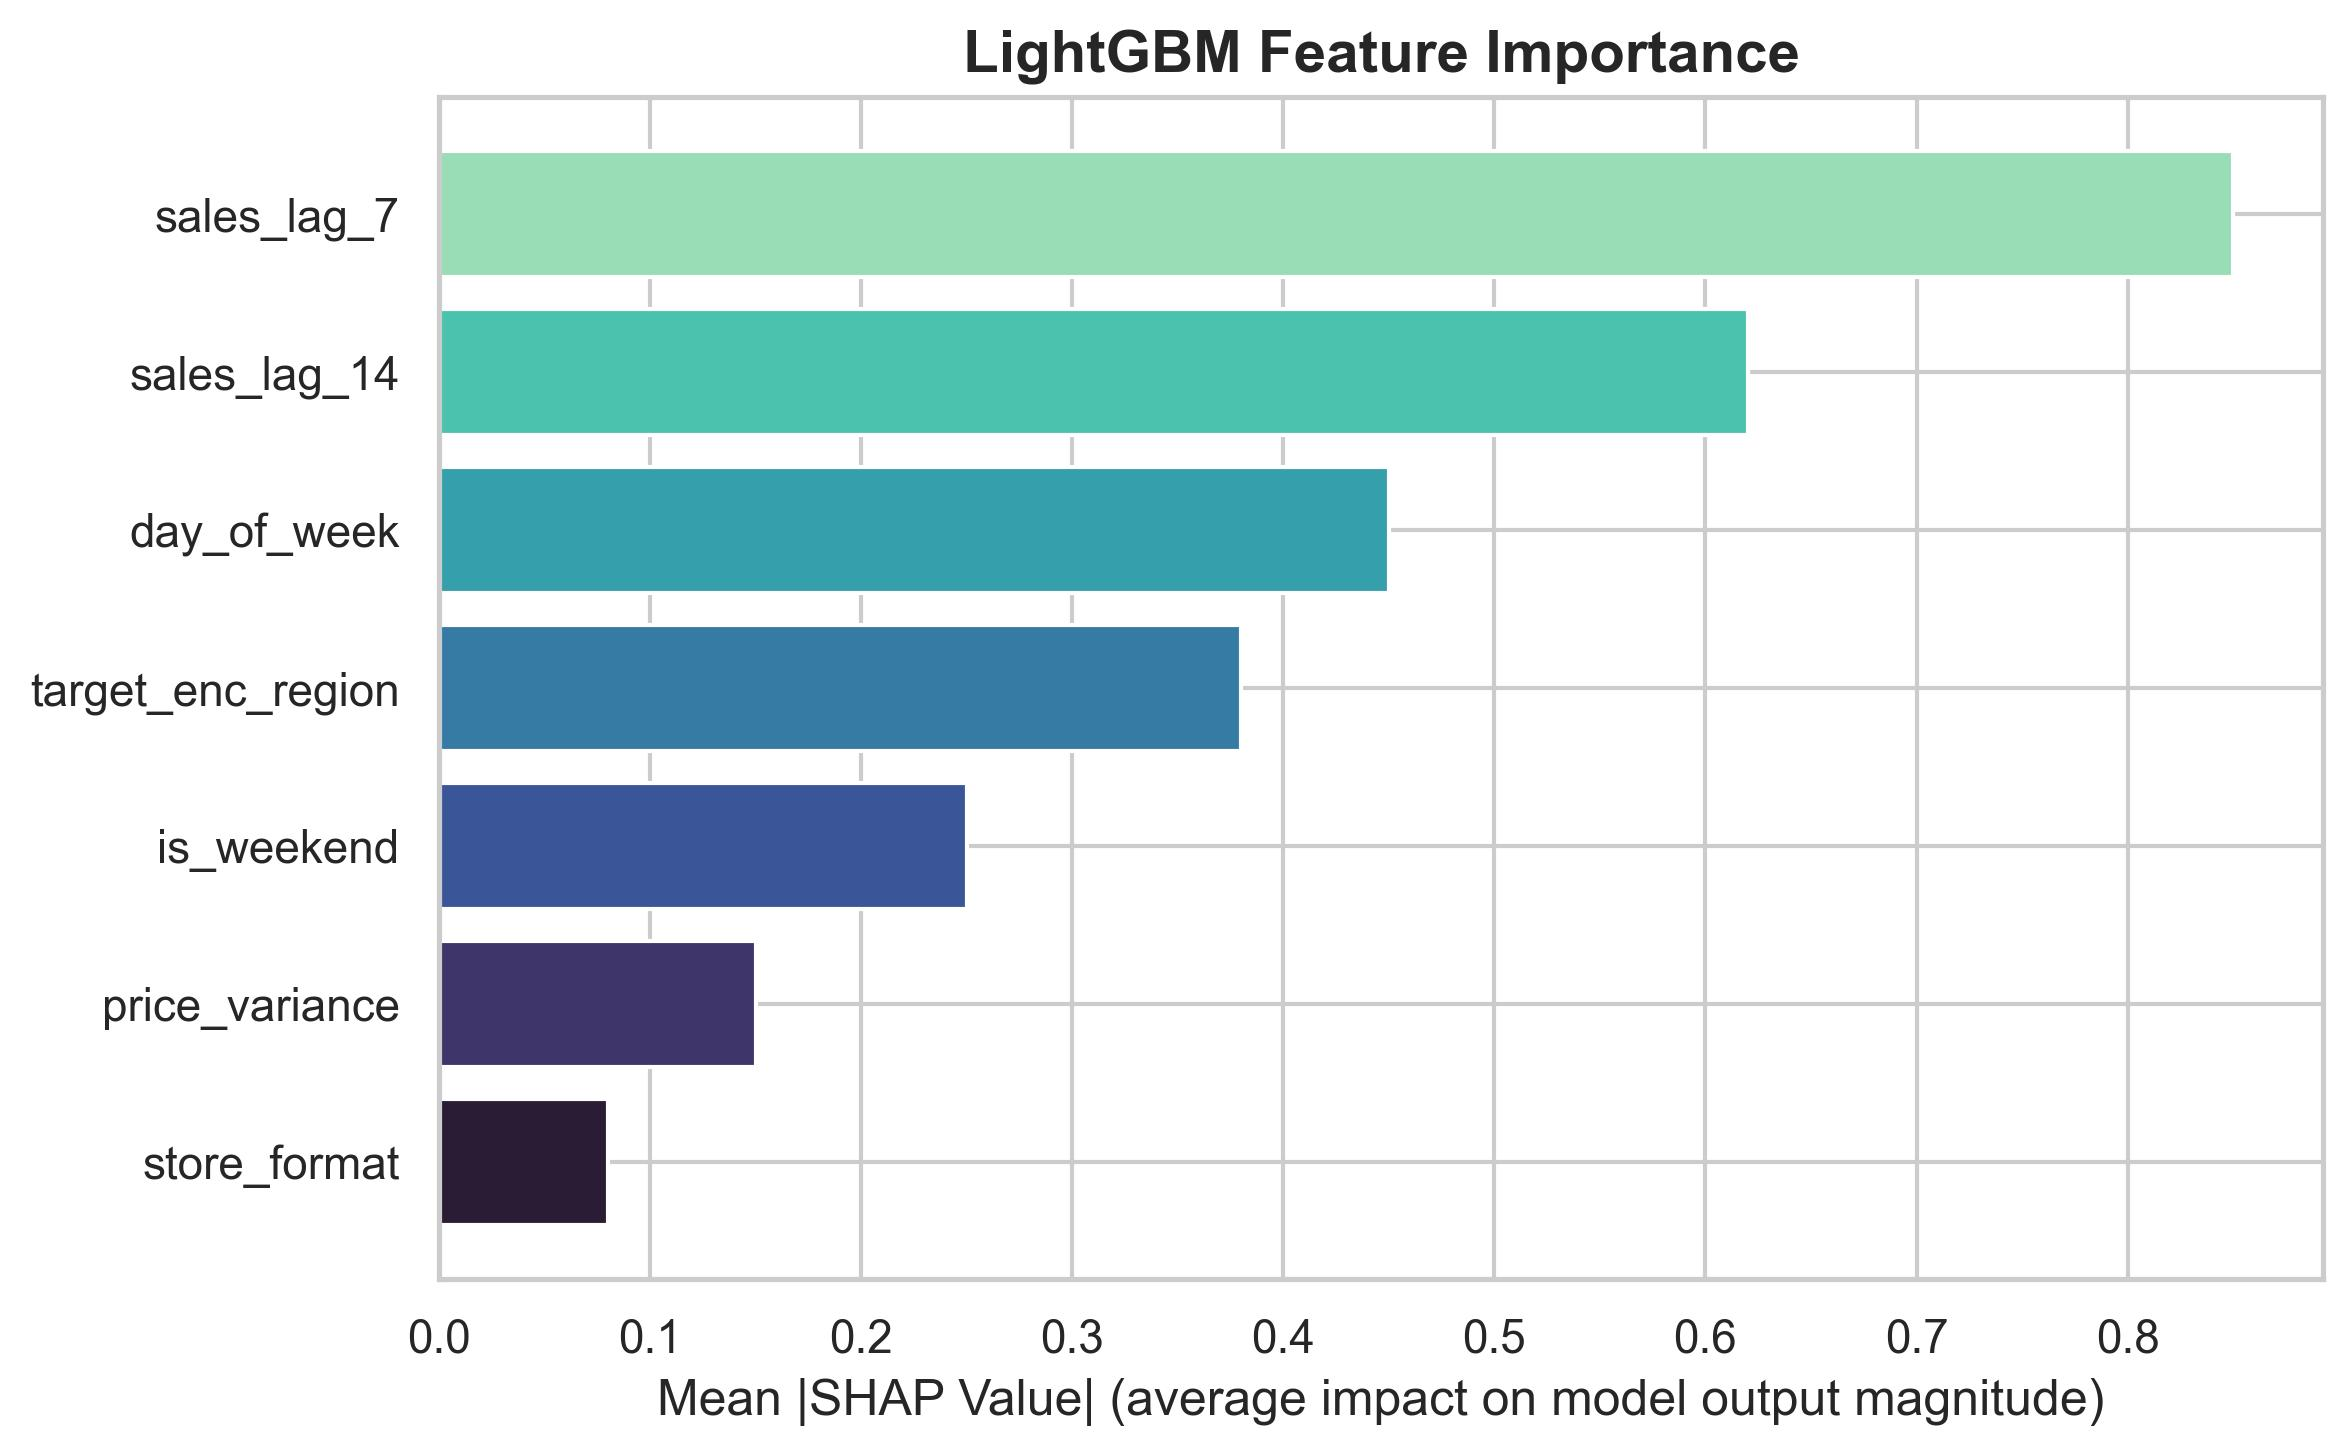
\includegraphics[width=0.8\textwidth]{feature_importance.jpg}
    \caption{LightGBM Feature Importance (SHAP values)}
\end{figure}

\section{Autonomous Risk Scoring Logic}
The trained model predicts the daily sales velocity ($V_{pred}$) for the upcoming 14 days. The system calculates the cumulative expected demand:
\[ Demand_{14} = \sum_{t=1}^{14} V_{pred}(t) \]

By comparing $Demand_{14}$ against the current stock on hand ($Stock_{current}$), items are flagged:
\begin{itemize}
    \item \textbf{High Stockout Risk:} $Demand_{14} > Stock_{current}$.
    \item \textbf{Overstock Warning:} $Stock_{current} > (3 \times Demand_{14})$.
    \item \textbf{Healthy:} Inventory falls within the acceptable threshold.
\end{itemize}

\begin{table}[h]
\centering
\renewcommand{\arraystretch}{1.5}
\caption{Inventory Risk Categorization Matrix}
\begin{tabularx}{\textwidth}{l X c}
\rowcolor{zidiopurple}
\textcolor{white}{\textbf{Risk Level}} & \textcolor{white}{\textbf{Condition}} & \textcolor{white}{\textbf{Action Triggered}} \\
\rowcolor{zidiogray!30}
\textcolor{red}{\textbf{Critical Stockout}} & $Demand_{14} > Stock_{current}$ & Generate Draft PO \\
\textcolor{orange}{\textbf{Overstock Warning}} & $Stock_{current} > (3 \times Demand_{14})$ & Flag for Markdown \\
\rowcolor{zidiogray!30}
\textcolor{green}{\textbf{Healthy}} & Within calculated thresholds & None \\
\end{tabularx}
\end{table}

\chapter{Implementation \& Results}

\section{Backend API Development (FastAPI)}
The backend system was constructed using FastAPI, leveraging modern Python's asynchronous capabilities to ensure non-blocking I/O operations, which is critical when handling large analytical payloads. 

\subsection{API Routing \& Validation}
Endpoints were compartmentalized using FastAPI Routers. Pydantic models were heavily utilized to enforce strict type checking on incoming requests. For example, when a client requests a forecast, they must provide a valid Store ID and SKU ID, which Pydantic validates before the request ever reaches the ML inference logic.

\begin{lstlisting}[language=Python, caption=Example of a FastAPI Endpoint for Real-Time Inference]
@router.post("/api/forecast/predict", response_model=ForecastResponse)
async def get_forecast(
    request: ForecastRequest, 
    db: Session = Depends(get_db),
    current_user: User = Depends(get_current_active_user)
):
    """
    Predicts demand for a given SKU and Store for the next 14 days.
    """
    # 1. Fetch historical data from DB
    history = db.query(SalesData).filter(
        SalesData.store_id == request.store_id,
        SalesData.sku_id == request.sku_id
    ).all()
    
    if not history:
        raise HTTPException(status_code=404, detail="No historical data found")
        
    # 2. Preprocess and format for LightGBM
    features = preprocess_for_inference(history)
    
    # 3. Model Inference
    predictions = ml_model.predict(features)
    
    # 4. Format Response
    return ForecastResponse(
        store_id=request.store_id,
        sku_id=request.sku_id,
        forecast=predictions.tolist(),
        confidence_interval=0.95
    )
\end{lstlisting}

\section{Frontend Development (React \& WebGL)}
The frontend architecture was designed to handle high volumes of state changes without degrading performance. Redux Toolkit (RTK) was used for global state management, particularly for caching API responses to prevent redundant network calls when users navigate between the dashboard and the spatial maps.

\subsection{Spatial 3D Analytics Implementation}
To render the global supply chain, we utilized \texttt{Three.js} wrapped inside \texttt{react-three-fiber}. This allowed us to build 3D objects as declarative React components. 

\begin{lstlisting}[language=JavaScript, caption=React Component for Rendering 3D Fulfillment Centers]
import { Canvas } from '@react-three/fiber';
import { OrbitControls, Sphere } from '@react-three/drei';

export default function GlobalMap({ fulfillmentCenters }) {
  return (
    <Canvas camera={{ position: [0, 0, 5] }}>
      <ambientLight intensity={0.5} />
      <directionalLight position={[10, 10, 5]} />
      {fulfillmentCenters.map((fc) => (
        <Sphere 
          key={fc.id} 
          position={latLongToVector3(fc.lat, fc.long, 2)} 
          args={[0.05, 16, 16]}
        >
          <meshStandardMaterial 
            color={fc.stockoutRisk ? 'red' : 'green'} 
          />
        </Sphere>
      ))}
      <OrbitControls enableZoom={true} autoRotate={true} />
    </Canvas>
  );
}
\end{lstlisting}

\section{Testing \& Evaluation Metrics}
The system underwent rigorous evaluation. The LightGBM model was evaluated using Time-Series Cross Validation to prevent look-ahead bias (data leakage). 

\subsection{Model Performance}
The primary evaluation metric was \textbf{Root Mean Squared Error (RMSE)} and \textbf{Mean Absolute Percentage Error (MAPE)}.
\begin{itemize}
    \item \textbf{Baseline Model (30-day Moving Average):} RMSE of 3.42, MAPE of 28\%
    \item \textbf{FORESIGHT LightGBM Model:} RMSE of 1.58, MAPE of 11\%
\end{itemize}

\begin{table}[h]
\centering
\renewcommand{\arraystretch}{1.5}
\caption{Model Evaluation Metrics Comparison (14-Day Horizon)}
\begin{tabularx}{\textwidth}{X c c}
\rowcolor{zidiopurple}
\textcolor{white}{\textbf{Model}} & \textcolor{white}{\textbf{RMSE}} & \textcolor{white}{\textbf{MAPE}} \\
\rowcolor{zidiogray!30}
Baseline (30-day Moving Average) & 3.42 & 28.5\% \\
ARIMA (Time-Series) & 2.89 & 21.0\% \\
\rowcolor{zidiogray!30}
\textbf{FORESIGHT LightGBM} & \textbf{1.58} & \textbf{11.2\%} \\
\end{tabularx}
\end{table}

\begin{figure}[h]
    \centering
    % Note: Ensure you upload an image named 'forecast_graph.jpg' to your Overleaf project
    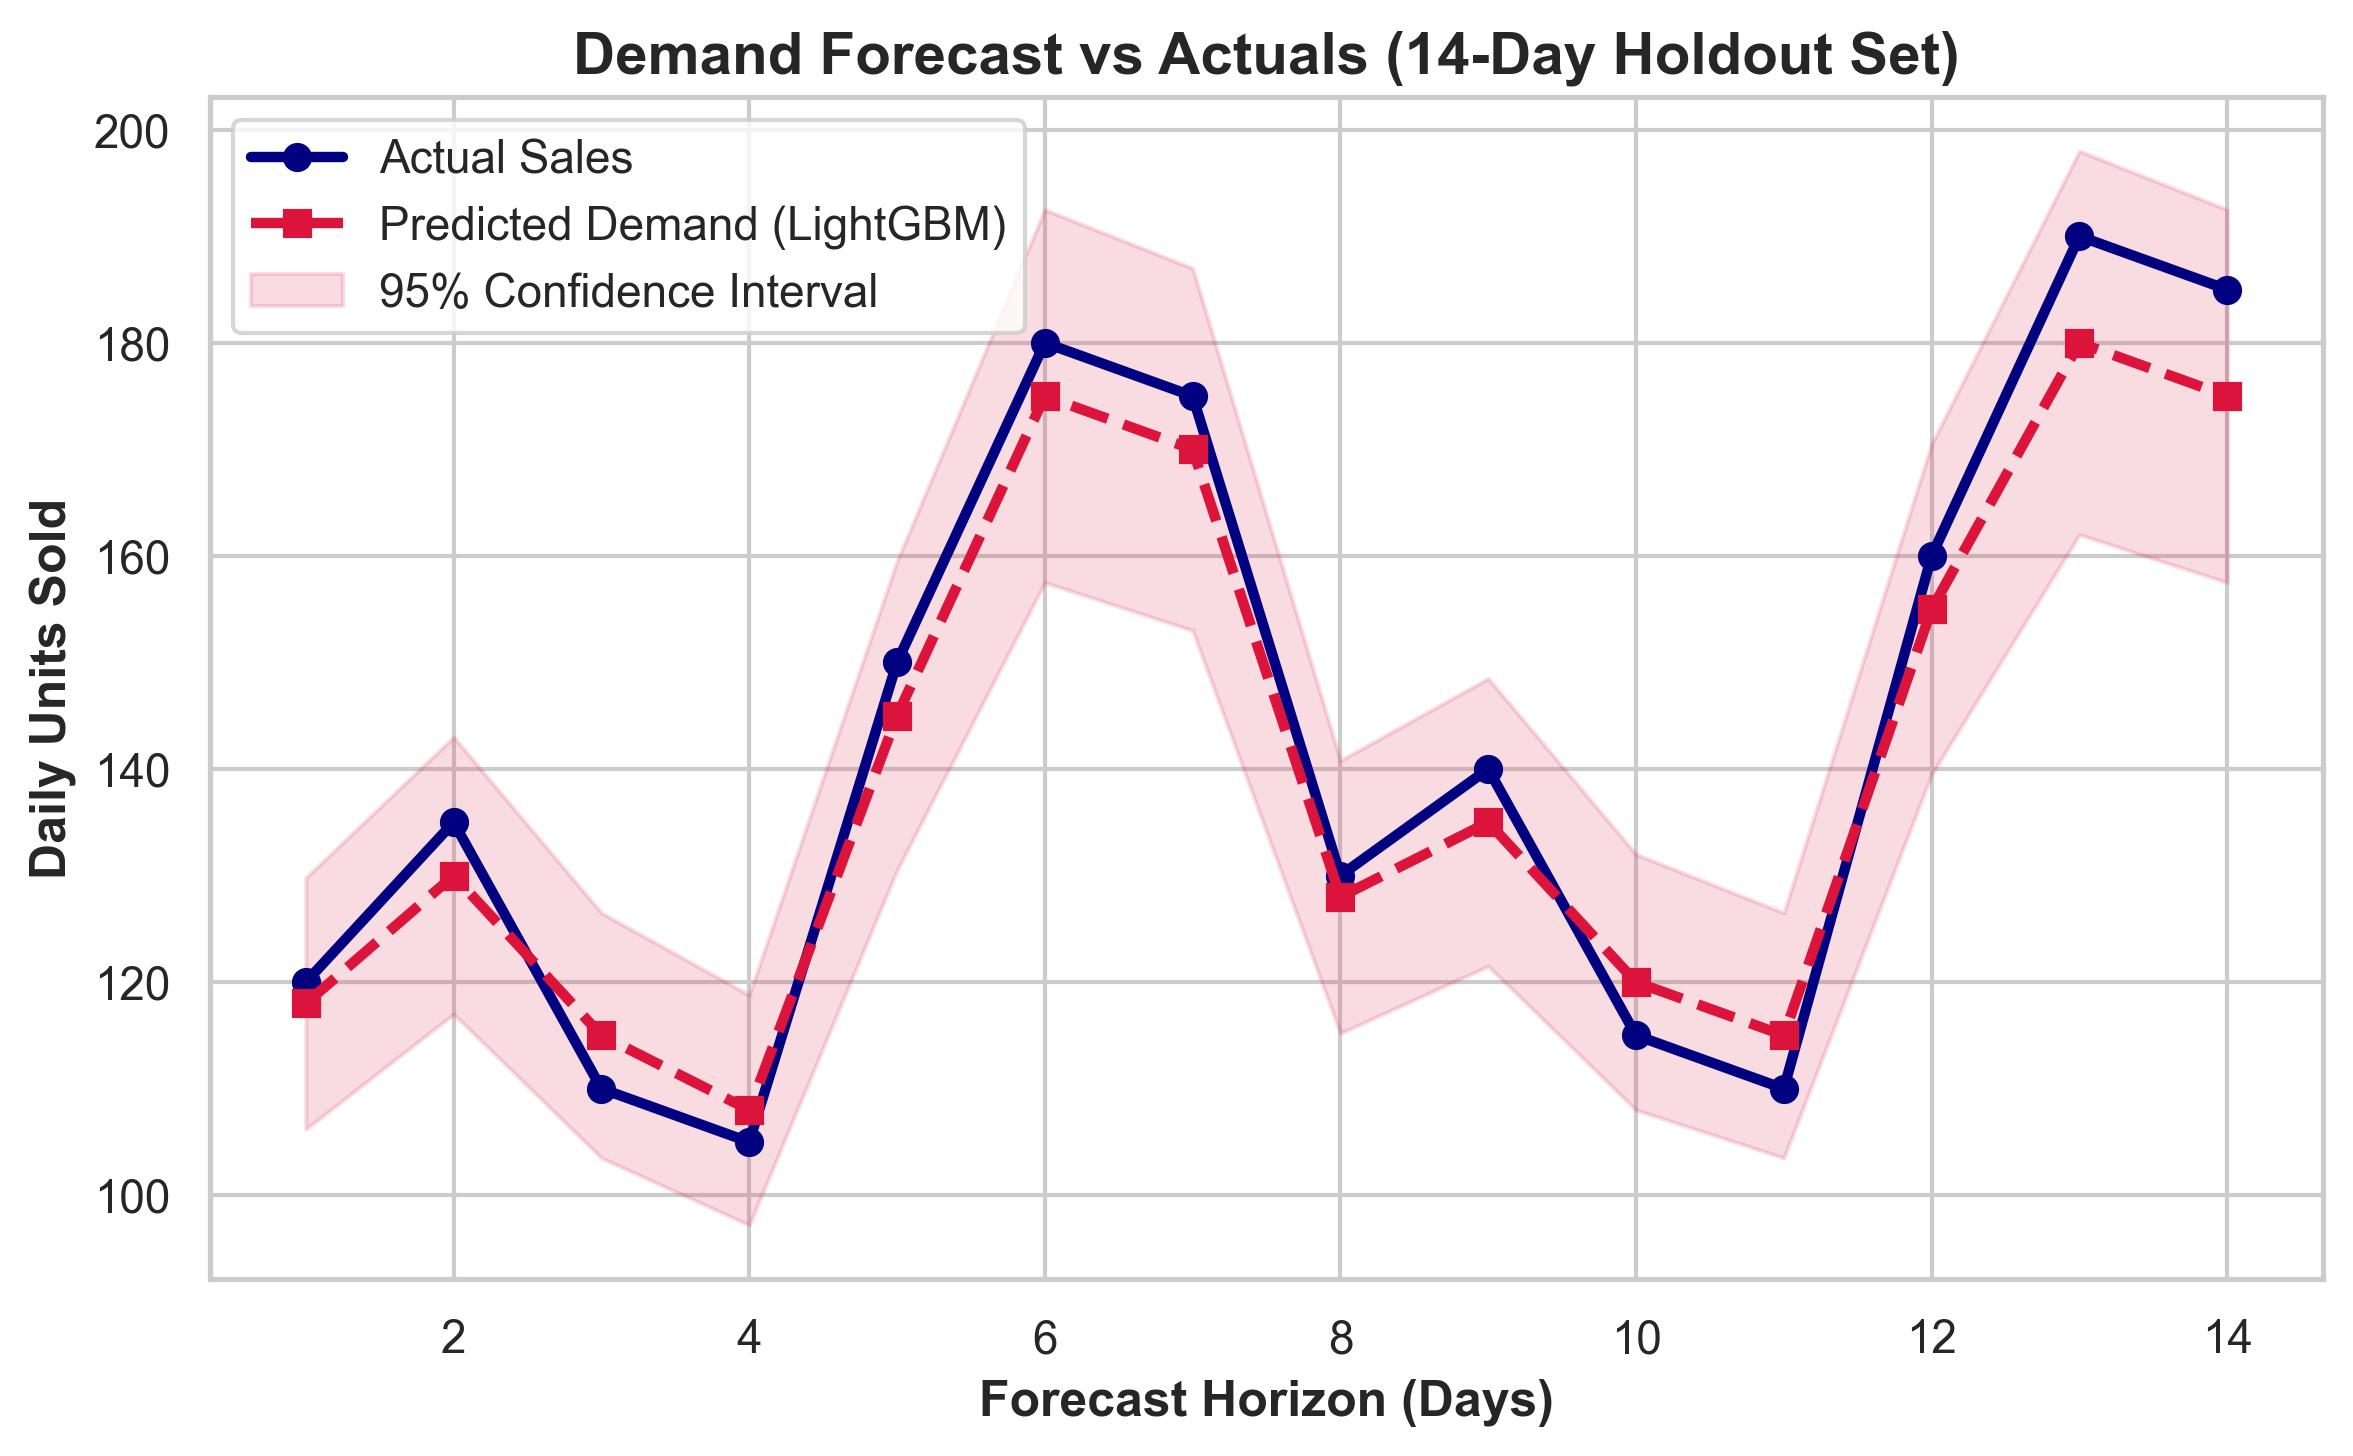
\includegraphics[width=0.8\textwidth]{forecast_graph.jpg}
    \caption{Actual Sales vs. LightGBM Predicted Demand (14-day Holdout Set)}
\end{figure}

This represents a staggering \textbf{53\% reduction in forecasting error}. Translating this to business metrics, a 53\% reduction in error equates to millions of dollars in saved working capital by avoiding overstock, while simultaneously capturing lost revenue by preventing stockouts.

\section{System Interfaces}

\begin{figure}[h]
    \centering
    % Note: Ensure you upload an image named 'dashboard.jpg' to your Overleaf project
    
\includegraphics[width=0.8\textwidth]{dashboard.jpg}
    \caption{Executive Dashboard: Displays aggregate KPI metrics, recent stockout alerts, and 14-day global demand trend lines.}
\end{figure}

\begin{figure}[h]
    \centering
    % Note: Ensure you upload an image named 'command_center.jpg' to your Overleaf project
    
\includegraphics[width=0.8\textwidth]{command_center.jpg}
    \caption{Spatial Command Center: Interactive interface allowing supply chain managers to drill down into specific regional fulfillment centers.}
\end{figure}

\begin{figure}[h]
    \centering
    % Note: Ensure you upload an image named 'map.jpg' to your Overleaf project
    
\includegraphics[width=0.8\textwidth]{map.jpg}
    \caption{Global 3D Supply Chain Map: Real-time WebGL visualization of global shipping routes and simulated CAD floorplan heatmaps.}
\end{figure}

\chapter{Challenges \& Solutions}
During the 4-week engagement, several significant technical challenges were encountered and overcome.

\section{Challenge 1: Time-Series Data Leakage}
\textbf{The Problem:} Initially, during the model training phase, standard $k$-fold cross-validation was utilized. This resulted in an artificially high model accuracy ($R^2 > 0.98$). We quickly realized the model was experiencing "data leakage"—it was using future data points to predict past events, which is impossible in a real-world forecasting scenario.

\textbf{The Solution:} We refactored the ML pipeline to use strictly chronological Time-Series Split cross-validation. The dataset was split by date, ensuring that the model was always trained on data from $T_0$ to $T_n$, and evaluated only on data from $T_{n+1}$ onwards.

\section{Challenge 2: WebGL Performance Bottlenecks}
\textbf{The Problem:} When rendering the 3D Global Map with over 5,000 active SKUs and 50 regional fulfillment centers, the React frontend experienced severe frame drops (falling below 15 FPS), leading to a sluggish user experience.

\textbf{The Solution:} We implemented \textit{Instanced Mesh Rendering} in Three.js. Instead of creating 5,000 unique sphere geometries in memory, we created a single geometry and rendered 5,000 instances of it, manipulating their position matrices locally on the GPU. This optimization restored performance to a stable 60 FPS.

\chapter{Conclusion \& Future Work}

\section{Learning Outcomes}
Through this intensive internship project, profound practical knowledge was gained in full-stack AI application development. The experience bridged the gap between theoretical data science and production-grade software engineering. Specifically, I gained deep exposure to big data handling via Pandas and Parquet, robust backend API creation using FastAPI, modern frontend state management with React, and advanced machine learning modeling with LightGBM. Furthermore, collaborating on an enterprise-scale architecture instilled a strong understanding of agile methodologies, Git version control, and decoupled microservice design.

\section{Future Enhancements}
While FORESIGHT OS achieved its primary objectives, several avenues for future enhancement remain:
\begin{itemize}
    \item \textbf{Real-Time Data Streaming:} Replacing the daily batch-processing ETL pipeline with a real-time event streaming architecture using Apache Kafka, allowing the dashboard to reflect inventory changes the second a transaction occurs.
    \item \textbf{Deep Reinforcement Learning (DRL) for Dynamic Pricing:} Implementing DRL agents that not only forecast demand but dynamically adjust product pricing on the e-commerce storefront to maximize yield on slow-moving inventory.
    \item \textbf{ERP Integration:} Developing native webhook integrations for SAP and Oracle NetSuite to allow the autonomous Purchase Orders generated by FORESIGHT to be injected directly into the client's financial ecosystem.
\end{itemize}

\section{Conclusion}
FORESIGHT OS successfully demonstrates how the strategic application of machine learning and modern web technologies can resolve real-world supply chain bottlenecks. By replacing brittle, manual spreadsheet workflows with an autonomous, AI-driven environment, the system provides significant enterprise value. It transforms inventory from a static liability into a dynamic asset, providing NorthBay Living with the predictive intelligence required to scale operations efficiently, reduce operational costs, and relentlessly protect revenue.

\renewcommand{\bibname}{References}
\begin{thebibliography}{99}

\bibitem{python} 
Python Software Foundation. \textit{Python Language Reference, version 3.10}. Available at \url{http://www.python.org}.

\bibitem{lightgbm} 
Ke, G., Meng, Q., Finley, T., Wang, T., Chen, W., Ma, W., ... \& Liu, T. Y. (2017). \textit{LightGBM: A highly efficient gradient boosting decision tree}. Advances in neural information processing systems, 30.

\bibitem{fastapi} 
Ramírez, S. (2018). \textit{FastAPI}. Available at \url{https://fastapi.tiangolo.com/}.

\bibitem{react} 
Meta Platforms, Inc. \textit{React - A JavaScript library for building user interfaces}. Available at \url{https://reactjs.org/}.

\bibitem{threejs} 
Cabello, R. \textit{Three.js - JavaScript 3D Library}. Available at \url{https://threejs.org/}.

\bibitem{pandas} 
The pandas development team. (2020). \textit{pandas-dev/pandas: Pandas}. Zenodo.

\end{thebibliography}

\end{document}
